\chapter{Model}
The estimation methods mentioned up to this point all estimate the whole network. 
One problem with this approach is that, for real world problems, the network size may be rather large. 
Especially so in the biomedical domain, where we might look at problems having only a few variables of interest (e.g. clinical factors such as the viral load of an HIV patient), though these might interact with a large number of other variables (e.g. known relevant mutations of patients). Instead of the whole network, we are often only concerned with the interactions that affect a few variables.
More specifically, we want to infer the Markov Blanket of the few nodes.
The Markov Blanket of a node is the set of nodes that when conditioned on, render its distribution independent of all the other nodes in the network.
For \gls{GGM}s (and other undirected graphical models) this is equivalent to the local Markov property. 
As such, the Markov Blanket of a node consists of the set of its direct neighbors in the graph (see \autoref{section:graphmodels}).
An example is given in \autoref{fig:MB_GGM}.

\begin{figure}[H]
	\centering
	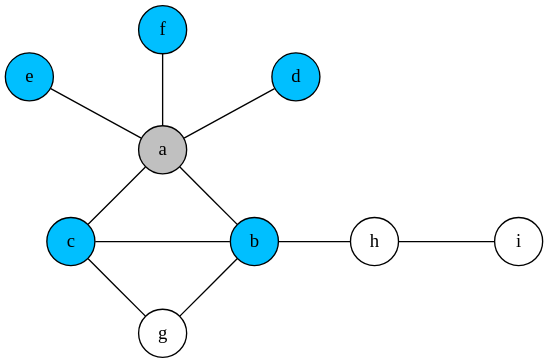
\includegraphics[width=0.5\textwidth]{MB_graph}
	\caption{The Markov Blanket of node 'a' consists of all blue nodes, as they are its direct neighbors.}
	
	\label{fig:MB_GGM}
\end{figure}

\citet{kaufmann_bayesian_2015} present an efficient Gibbs sampler for inferring the Markov Blanket for a small number of variables.
While following an approach similar to \citet{wang_bayesian_2012}, 
a conditional independence property in the likelihood is used for separating the inference of the Markov Blanket from the rest of the network.
Due to the reliance on computationally expensive \gls{MCMC} methods for the estimation, this is a highly useful property and makes the Bayesian approach to Covariance Selection feasible for bigger problem sizes (in terms of total network size).


In this Chapter we will provide an overview of \citet{kaufmann_bayesian_2015} and its most important properties.
The full model and its derivation are omitted for the sake of brevity and can be found in \autoref{A:model}.
Furthermore, we extend the sampler with Simulated Annealing for estimating the MAP instead of the whole posterior marginals.


\section{Bayesian Markov Blanket}
We stay in the setting of Gaussian Graphical Models.
Let $\W \in \mathbb{R}^{(p+q)}$ be a symmetric positive definite matrix.
Data $\matr{X}$ is assumed to be normally distributed with
$$
\matr{X} \sim \mathcal{N}_{(p+q)}(0,\W^{-1})
$$ 
Additionally, the observed data $X=(\matr{x_1}, \dots, \matr{x_{(p+q)}})$ with $\matr{x}_i\in\mathbb{R}^{n}$ is ordered such that the first $p$ columns correspond to query variables we are interested in, with $q$ corresponding to the remaining variables.
It is assumed that $p\ll q$.
Furthermore, $\matr{S}$ and $\matr{W}$ are partitioned into block matrices according to $p$ and $q$:
\begin{equation*}
\matr{W}=
\raisebox{0.3\baselineskip}{$
	\begin{blockarray}{ccc}
	p & q& \\
	\begin{block}{(cc)l}
	\matr{W}_{11} & \matr{W}_{12}&p \\
	\matr{W}_{12}^T & \matr{W}_{22}&q \\
	\end{block}
	\end{blockarray}
	$}
\quad \quad \quad \quad 
\matr{S}=
\raisebox{0.3\baselineskip}{$
	\begin{blockarray}{ccc}
	p & q& \\
	\begin{block}{(cc)l}
	\matr{S}_{11} & \matr{S}_{12}&p \\
	\matr{S}_{12}^T & \matr{S}_{22}&q \\
	\end{block}
	\end{blockarray}
	$}
\end{equation*}

The Markov Blanket of the query variables $p$ is now given by the block $\Wxy$.
As such, the aim is to estimate the precision matrix block $\Wxy$.
It is important to note that $\Sxx$ and $\Wxx$ are much smaller than $\Syy$ and $\Wyy$ respectively (given $p\ll q$).

The main motivation of the \gls{BMB} sampler is a block-wise factorization of the likelihood that effectively allows decoupling the inference of $\Wxy$ from the large matrix $\Wyy$.
By then constructing a prior admitting a similar factorization, the factorization can be propagated to the posterior which then reveals a block-wise conditional independence structure.

\subsection{Likelihood}
Let the sample Covariance be $\matr{S} = \matr{X}^T\matr{X}$.
As shown in \autoref{GRAPH_SELECTION}, the likelihood is of form
\begin{equation}
\label{eq:BMB_likelihood}
p(\matr{S}|\W) \propto \det(\matr{W}^{n/2}) \exp\tr\Big(-\frac{1}{2} \matr{WS}\Big)
\end{equation}
 which corresponds to a Wishart distribution:
$$
p(\matr{S}|\W) \propto \mathcal{W}_{p+q}(n,\matr{W})
$$
\citet{kaufmann_bayesian_2015} then show that the likelihood factorizes as shown in Lemma \autoref{lemma:ll}.

\begin{tcolorbox}[colback=yellow!5!white,colframe=yellow!75!black]
	\begin{customlemma}{1}[\cite{kaufmann_bayesian_2015}]
		\label{lemma:ll}
		Let $\Wyys = \Wyy - \Wyx\Wxx^{-1}\Wxy$ be the Schur complement of block $\Wxx$ in $\W$.
		Then the likelihood of the covariance matrix factorizes in terms of $\W$ as follows:
		$$
		\mathcal{L}_S(\matr{W}) \propto \mathcal{L}_1(\Wxx, \Wxy)\mathcal{L}_2(\Wyys)
		$$
	\end{customlemma}
\end{tcolorbox}
It should be noted that when seen as a function of $\W$, the likelihood is no proper \gls{pdf} 
\footnote{The integral of the likelihood over $\W$ is not equal to one: $\int \mathcal{L}_S(\matr{W}) \dif\W \neq 1$} 
and the factorization is as such only a functional statement.

We will not prove this factorization here but rather assume it, for constructing a prior. 
Subsequently the factorization can be shown in the full posterior.
This results in an arguably less convoluted derivation.

\subsection{Prior}
The prior for $\W$ has to ensure symmetry and positive-definiteness.
Consequently, a Wishart prior is chosen.
It is the natural conjugate prior to $p(\matr{S}|\matr{W})$ with its support being symmetric positive definite matrices.
But the Wishart alone is insufficient, as sparsity is to be enforced. 
For this, a \gls{DE} prior for the non-diagonal entries of $\matr{W}$ can be used.
To admit a block-wise factorization similar to the likelihood, the \gls{DE} prior is only placed on the non-diagonal entries of the $\Wxy$ block.
Analogous to \citet{wang_bayesian_2012}, the \gls{DE} prior is represented as a scale mixture of Gaussians (see \autoref{BGLASSO}) with inverse-Gaussian distributed scale parameters $\matr{T}=\{t_{ij}\}$.
\begin{align}
\label{eq:BMB_prior}
P(\matr{W}|\matr{T}) &=
\mathcal{W}_{p+q} \big(p + q + 1, \matr{I}\big) p(\matr{W}_{12} | \matr{T} )
\\
&\propto \exp\tr \Big(-\frac{1}{2} \matr{W}\Big)
\prod_{{\substack{i=1,\dots,p\\j=1,\dots,q}} }   \frac{1}{\sqrt{2\pi \matr{T}_{ij}}} \exp 
\Big( - \frac{(\matr{W}_{12})_{ij}^2}{2\matr{T}_{ij}} \Big) 
\nonumber\\ \nonumber\\
P(\matr{T}| \lambda) &\propto
\prod_{{\substack{i=1,\dots,p\\j=1,\dots,q}} }   \frac{\lambda^2}{2} \exp \Big( - \frac{\lambda^2}{2} \matr{T}_{ij} \Big)
\nonumber
\end{align}

\subsection{Factorization of the Posterior}
The joint distribution of the model arises from combining the compound prior in \autoref{eq:BMB_prior} with the likelihood given in \autoref{eq:BMB_likelihood}.

\begin{align*}
p(\matr{W}, \matr{S}, \matr{T} | \lambda) =& p(\matr{W}_{11}, \matr{W}_{12}, \matr{W}_{22}, \matr{S}, \matr{T} | \lambda) \\
\propto &\det(\matr{W})^{\frac{n}{2}}  \det(\matr{S})^{\frac{n-(p+q)-1}{2}} 
\\
&\exp\Bigg(-\frac{1}{2} \tr [\matr{WS}+\matr{W}] - \frac{1}{2} \sum_{{\substack{i=1,\dots,p\\j=1,\dots,q}} } \frac{(\matr{W}_{12})_{ij}^2}{\matr{T}_{ij}}  \Bigg) 
\\
&\times \Big[\prod_{{\substack{i=1,\dots,p\\j=1,\dots,q}} }  \frac{1}{\sqrt{2\pi \matr{T}_{ij}}}\Big]
p(\matr{T}|\lambda)
\end{align*}

Let the Schur complement of $\matr{W}_{11}$ in $\W$ be:
$$\matr{W}_{22.1} = \matr{W}_{22} - \matr{W}_{12}^T \matr{W}_{11}^{-1} \matr{W}_{12}$$

We can reparameterize the joint distribution by $(\matr{W}_{11}, \matr{W}_{12}, \matr{W}_{22.1})$, with the change of variable admitting a constant Jacobian:
$$ J\big((\matr{W}_{11}, \matr{W}_{12}, \matr{W}_{22}) \rightarrow (\matr{W}_{11}, \matr{W}_{12}, \matr{W}_{22.1})\big) = \matr{1} $$

With the new parameterization, the determinants and traces can be written as:
\begin{align*}
\det(\matr{W}) &= \det(\matr{W}_{11}) \det(\matr{W}_{22} - \matr{W}_{12}^T \matr{W}_{11}^{-1}\matr{W}_{12})
\\
&= \det(\matr{W}_{11}) \det(\matr{W}_{22.1})
\\
\\
\tr(\matr{WS}) &= \tr\big[\matr{W}_{11}\matr{S}_{11} + \matr{W}_{12}\matr{S}_{21} + \matr{W}_{21}\matr{S}_{12} + \matr{W}_{22}\matr{S}_{22}   \big]
\\
&= \tr\big[\matr{W}_{11}\matr{S}_{11} + \matr{W}_{12}\matr{S}_{12}^T + \matr{W}_{12}^T\matr{S}_{12} + (\matr{W}_{22.1} + \matr{W}_{12}^T\matr{W}_{11}^{-1}\matr{W}_{12}) \matr{S}_{22}   \big]
\\
&= \tr\big[
\Cline[blue]{\matr{W}_{11}\matr{S}_{11}} + 
\Cline[yellow]{\matr{W}_{12}\matr{S}_{12}^T + 
	\matr{W}_{12}^T\matr{S}_{12}} + 
\Cline[red]{\matr{W}_{22.1}\matr{S}_{22}} + 
\Cline[green]{\matr{W}_{12}^T\matr{W}_{11}^{-1}\matr{W}_{12}\matr{S}_{22}}   
\big]
\\
\\
\tr(\matr{W}) &= \tr(\matr{W}_{11}) + \tr(\matr{W}_{22})
\\
&= \tr(\Cline[blue]{\matr{W}_{11}}) + 
\tr(\Cline[red]{\matr{W}_{22.1}}) +
\tr(\Cline[green]{\matr{W}_{12}^T\matr{W}_{11}^{-1}\matr{W}_{12}})
\end{align*}
When plugged into the joint distribution, this results in:
\begin{align*}
p(\matr{W}_{11}, \matr{W}_{12}, &\matr{W}_{22.1}, \matr{S}, \matr{T} | \lambda) \propto
\\
&\det(\matr{W}_{11})^{n/2} \det(\matr{W}_{22.1})^{n/2} \det(\matr{\matr{S}})^{\frac{n-(p+q)-1}{2}}
\\
\times& \exp \Big(
-\frac{1}{2}
\tr\big[
\Cline[blue]{\matr{W}_{11} (\matr{S}_{11} + \matr{I}) }+ 
\Cline[red]{\matr{W}_{22.1}  (\matr{S}_{22} + \matr{I})} + 
\\
&\quad \quad \quad \quad \quad \quad
\Cline[yellow]{2 (\matr{W}_{12}^T\matr{S}_{12})} +
\Cline[green]{
	\matr{W}_{12}^T \matr{W}_{11}^{-1}\matr{W}_{12} 
	(\matr{S}_{22} + \matr{I})}
\big]
\Big)
\\
\times& \exp\Big(- \frac{1}{2} \sum_{{\substack{i=1,\dots,p\\j=1,\dots,q}} } \frac{(\matr{W}_{12})_{ij}^2}{\matr{T}_{ij}} \Big) \quad \Big[\prod_{{\substack{i=1,\dots,p\\j=1,\dots,q}} }  \frac{1}{\sqrt{2\pi \matr{T}_{ij}}}\Big]
\quad
p(\matr{T}|\lambda)
\\\\
%%%%%%%%%%%%%%%%%%%%%%%%%%%%%%%%%%%%%%%%%%%%%%%%%%%%%%%%%%%%%%%%%%%%%%%%%%%
=&\det(\matr{W}_{11})^{n/2} \det(\matr{\matr{S}})^{\frac{n-(p+q)-1}{2}} 
\\
\times& \exp \Big(
-\frac{1}{2}
\tr\big[
\Cline[blue]{\matr{W}_{11} (\matr{S}_{11} + \matr{I}) } +  
\Cline[yellow]{2 (\matr{W}_{12}^T\matr{S}_{12})} +
\Cline[green]{
	\matr{W}_{12}^T \matr{W}_{11}^{-1}\matr{W}_{12} 
	(\matr{S}_{22} + \matr{I})}
\big]
\Big)
\\
\times& \exp\Big(- \frac{1}{2} \sum_{{\substack{i=1,\dots,p\\j=1,\dots,q}} } \frac{(\matr{W}_{12})_{ij}^2}{\matr{T}_{ij}} \Big) \quad \Big[\prod_{{\substack{i=1,\dots,p\\j=1,\dots,q}} }  \frac{1}{\sqrt{2\pi \matr{T}_{ij}}}\Big]
\quad
p(\matr{T}|\lambda)
\\
\times& 
	\det(\matr{W}_{22.1})^{n/2} 
	\exp
	\Bigg(
		-\frac{1}{2}
		\tr
		\Big[
			\Cline[red]{\matr{W}_{22.1}  (\matr{S}_{22} + \matr{I})}
		\Big]
	\Bigg)
\end{align*}
In this formulation it's clear to see that by conditioning on $\Syy$, $\Wyys$ is (conditionally) independent of $\Wxx$ and $\Wxy$.
\begin{tcolorbox}[colback=red!5!white,colframe=red!60!black, title=Conditional Independence Property]
	The posterior distribution of $\W$ factorizes as follows:
	\begin{equation}
	p(\matr{W}_{11}, \matr{W}_{12}, \matr{W}_{22.1}, \matr{T} | \matr{S}, \lambda)
	= p(\matr{W}_{11}, \matr{W}_{12}, \matr{T} | \matr{S}, \lambda) p(\matr{W}_{22.1} | \matr{S}, \lambda) 
	\end{equation}
	This implies that the posterior of $(\Wxx, \Wxy)$ is conditionally independent of $\Wyys$, given $\matr{S}$:
	\begin{equation}
	\label{eq:W22}
	(\Wxx \text{,} \Wxy)\bigCI \Wyys | \matr{S}
	\end{equation}
\end{tcolorbox}
As a consequence, the Markov Blanket can be inferred independently of the prohibitively large $\Wyy$, using only the  joint posterior over $\Wxx$, $\Wxy$ and $\matr{T}$.

%The joint posterior over $\Wxx$, $\Wxy$ and $\matr{T}$ is then:
\begin{tcolorbox}[colback=red!5!white,colframe=red!60!black, title=Joint Posterior Distribution]
	\begin{align}
	\label{eq:jointpost}
		p(\matr{W}_{11}, \matr{W}_{12}, \matr{T} | \matr{S}, \lambda)
		\propto& \quad
		\det(\matr{W}_{11})^{n/2} \exp \Big( - \frac{1}{2} \tr\big[ \matr{W}_{11} (\matr{S}_{11} + \matr{I}) \big]\Big)
		\\
		&\times \exp\Bigg(
		-\frac{1}{2}\text{vec}(\matr{W}_{12})^T \Big[
		(\matr{S}_{22} + \matr{I}) \otimes \matr{W}_{11}^{-1} +\matr{D}\Big]\text{vec}(\matr{W}_{12})
		\nonumber\\&\quad \quad  \quad \quad \quad \quad 
		- \text{vec}(\matr{W}_{12})^T \text{vec}(\matr{S}_{12})
		\Bigg)
		\nonumber \\
		&\times \Big[\prod_{{\substack{i=1,\dots,p\\j=1,\dots,q}} }  \frac{1}{\sqrt{2\pi \matr{T}_{ij}}}\Big]
		p(\matr{T}|\lambda)
		\nonumber
	\end{align}
	Where $\matr{D} = \text{diag}(\text{vec}(\matr{T}))^{-1}$,
	i.e. $\matr{D}$ is a diagonal matrix with entries $(\matr{T}_{ij})^{-1}$.
\end{tcolorbox}

\subsection{Posterior Conditionals}

It can now be shown that each of the posterior conditionals of $\Wxx$, $\Wxy$, $\matr{T}$ and $\Wyys$ follows a known closed-form distribution.
While we may not be interested in $\Wyys$ (or $\Wyy$) directly,
it is required for embedding the \gls{BMB} in the copula sampler.

The resulting distributions are shown in the following overview, while the full derivation can be found in \autoref{A:post_cond}.
They are omitted at this point of the thesis for the sake of compactness.

\begin{tcolorbox}[colback=red!5!white,colframe=red!60!black, title= Posterior Conditional of $\Wxy$]
	\begin{enumerate}
		\item $\Wxy$ follows a multivariate Normal distribution:
		\begin{align}
		\text{vec}(\matr{W}_{12}) | \matr{W}_{11}, \matr{T}, \matr{S}, \lambda &\sim \mathcal{N}(-\matr{C}^{-1} \text{vec}(\matr{S}_{12}), \matr{C}^{-1})
		\\
		\matr{C} = \Big[
		(\matr{S}_{22} + \matr{I}) &\otimes \matr{W}_{11}^{-1} +\matr{D}\Big]
		\nonumber
		\end{align}
		With $\matr{D} = \text{diag}(\text{vec}(\matr{T}))^{-1}$\\
		It should be noted, that as a special case for $\matr{T}_{ij} \rightarrow \infty$, i.e.
		$\matr{D}\rightarrow \matr{0}$ the posterior simplifies to:
		$$
		\mathcal{N}\Big(-\text{vec}(\Wxx \Sxy (\Syy+\matr{I}) ^{-1}), 
		(\Syy + \matr{I})^{-1} \otimes \Wxx
		\Big)
		$$
		\item $\Wxx$ follows a \gls{MGIG} distribution:
		\begin{align}
		\Wxx | \Wxy, \matr{T}, \matr{S}, \lambda \sim 
		\mathcal{MGIG}_B
		\Big(
		\frac{n+p+1}{2}, \ 
		\Sxx+\matr{I},\  
		\Wxy(\Syy+I)\Wxy^T
		\Big)
		\end{align}
		(Using the parametrization of the \gls{MGIG} as presented by \citet{butler_generalized_1998})
		\item $\Wyys$ follows a Wishart distribution:
		\begin{align}
		\Wyys | \matr{S}, \lambda \sim \mathcal{W}\Big(
		n-\frac{p-1}{3}, \Syy
		\Big)
		\end{align}
		\item $(\matr{T}_{ij})^{-1}$ follow an inverse Gaussian distribution:
		\begin{align}
		(\matr{T}_{ij})^{-1} \sim \mathcal{IG}
		\Big(
		\mu' = \sqrt{
			\frac{\lambda^2}{(\matr{W}_{12})_{ij}^2}
		},
		\lambda' = \lambda^2
		\Big)
		\end{align}
	\end{enumerate}		
\end{tcolorbox}

While $\Wxy$, $\Wyys$ and $\matr{T}$ follow distributions that can be easily sampled, the \gls{MGIG} is more difficult.
\citet{bernadac_random_1995} shows that the \gls{MGIG} can be represented and sampled as a continued fraction of Wishart distributed Matrices.
But by its very nature, continued fractions of matrices are numerically unstable.
Consequently, finding an alternative representation of the posterior that does not rely on the \gls{MGIG} is favored.


\subsubsection{Posterior Marginal of $\Wxx$}
\label{ss:postmarginal}
The joint posterior of $\Wxx$ and $\Wxy$ can be split up using the chain rule:
$$ p(\Wxx, \Wxy | \matr{T}, \matr{S}, \lambda) = 
p(\Wxy | \Wxx, \matr{T}, \matr{S}, \lambda) p(\Wxx | \matr{T}, \matr{S}, \lambda)
$$
From the previous section, it is known that the posterior conditional of $\Wxy | \Wxx, \matr{T}, \matr{S}, \lambda$
is proportional to the exponential part of a normal distribution (for details see \autoref{A:post_cond}).
The marginal $p(\matr{W}_{11} |  \matr{T}, \matr{S}, \lambda)$ can then be computed by integrating out $\Wxy$.

For this step we utilize the fact that integrating over the unnormalized part of a Gaussian distribution results in its normalization constant. This is given by construction, since a \gls{pdf} has to integrate to one.
\begin{align*}
\int \mathcal{N}(x;\mu, \matr{\Sigma})\dif x=
&\int \frac{1}{\sqrt{(2\pi)^n\det(\boldsymbol\Sigma)}}
\exp\left(
-\frac{1}{2}({x}-{\mu})^T{\boldsymbol\Sigma}^{-1}({x}-{\mu})
\right)
\dif x
= 1
\\
\Rightarrow
&\int
\exp\left(
-\frac{1}{2}({x}-{\mu})^T{\matr{\Sigma}}^{-1}({x}-{\mu})
\right)
\dif x
= \sqrt{(2\pi)^n\det(\matr{\Sigma})}
\\
&\qquad\qquad\qquad\qquad\qquad\qquad\qquad\quad\quad\ 
\propto \sqrt{\det(\matr{\Sigma})}
\end{align*}

Now plugging the joint posterior \autoref{eq:jointpost} into the marginalization results in:
\begin{align*}
	 p(&\matr{W}_{11} |  \matr{T}, \matr{S}, \lambda)=\int p(\matr{W}_{11}, \matr{W}_{12} |  \matr{T}, \matr{S}, \lambda)\dif\Wxy
	\\
	&\propto 
	\int
	\det(\matr{W}_{11})^{n/2} \exp \Big( - \frac{1}{2} \tr\big[ \matr{W}_{11} (\matr{S}_{11} + \matr{I}) \big]\Big)
	\\
	&\times \exp\Bigg(
	-\frac{1}{2}\text{vec}(\matr{W}_{12})^T \Big[
	(\matr{S}_{22} + \matr{I}) \otimes \matr{W}_{11}^{-1} +\matr{D}\Big]\text{vec}(\matr{W}_{12})
	- \text{vec}(\matr{W}_{12})^T \text{vec}(\matr{S}_{12})
	\Bigg)
	\dif\Wxy
	\\\\
	&= 
	\det(\matr{W}_{11})^{n/2} \exp \Big( - \frac{1}{2} \tr\big[ \matr{W}_{11} (\matr{S}_{11} + \matr{I}) \big]\Big)
	\\
	&\times 
	\int
	\underbrace{
		\exp\Bigg(
		-\frac{1}{2}\text{vec}(\matr{W}_{12})^T \Big[
		(\matr{S}_{22} + \matr{I}) \otimes \matr{W}_{11}^{-1} +\matr{D}\Big]\text{vec}(\matr{W}_{12})
		- \text{vec}(\matr{W}_{12})^T \text{vec}(\matr{S}_{12})
		\Bigg)
	}_{\propto\mathcal{N}\big(-\matr{C}^{-1}\text{vec}(\Wxy), \matr{C}^{-1}\big)}
	\dif\Wxy		
	\\\\
	&\propto 
	\det(\matr{W}_{11})^{n/2} \exp \Big( - \frac{1}{2} \tr\big[ \matr{W}_{11} (\matr{S}_{11} + \matr{I}) \big]\Big)
	{\det(\matr{C})^{\frac{1}{2}}}
\end{align*}
\begin{tcolorbox}[colback=red!5!white,colframe=red!60!black, title=
	Posterior Marginal $\Wxx|\matr{T}\text{,}\matr{S}\text{,}\lambda$]
	\begin{equation*}
	p(\matr{W}_{11} |  \matr{T}, \matr{S}, \lambda)= 
	\det(\matr{W}_{11})^{n/2} \exp \Big( - \frac{1}{2} \tr\big[ \matr{W}_{11} (\matr{S}_{11} + \matr{I}) \big]\Big)
	\det
	\Big(
	(\matr{S}_{22} + \matr{I}) \otimes \matr{W}_{11}^{-1} +\matr{D}
	\Big)^{\frac{1}{2}}
	\end{equation*}
\end{tcolorbox}

To our knowledge, this offers no possibility of reformulation into some known closed-form distribution,
as the determinant arising from the normalization of $p(\Wxy | \Wxx, \matr{T}, \matr{S}, \lambda)$ cannot be split up.

For the special case $\matr{T}_{ij}\rightarrow0$, i.e. $\matr{D}\rightarrow\matr{0}$:
$$
\matr{C}\overset{D\rightarrow\matr{0}}{\rightarrow}
\big(
	(\Syy+I) \otimes \Wxx^{-1}
\big)
$$
\begin{align*}
\det
\Big(
	(\matr{S}_{22} + \matr{I}) \otimes \matr{W}_{11}^{-1}
\Big)^{\frac{1}{2}}
&\overset{\text{\tiny{(516 Matr. Cookbook)}}}{=}
\Big(
	\det(\Syy + \matr{I})^{\text{rank}(\Wxx^{-1})} 
	\det(\matr{W}_{11}^{-1})^{\text{rank}(\Syy+\matr{I})}
\Big)^{\frac{1}{2}}
\\
&=
\Big(
\det(\Syy + \matr{I})^{p} 
\det(\matr{W}_{11}^{-1})^{q}
\Big)^{\frac{1}{2}}
\\
&= 
\det(\Syy + \matr{I})^{\frac{p}{2}} 
\det(\matr{W}_{11})^{-\frac{q}{2}}
\end{align*}
As $\Wxx$  and $\Syy$ are symmetric positive definite matrices, they have full rank $p$ and $q$ respectively. 
It then also follows that $\text{rank}(\Syy + \matr{I})= \text{rank}(\Syy)$.

Then
\begin{align*}
 p(\matr{W}_{11} |  \matr{T}, \matr{S}, \lambda)
 &\overset{\matr{D}\rightarrow\matr{0}}{\propto}
\det(\matr{W}_{11})^{n/2} \exp \Big( - \frac{1}{2} \tr\big[ \matr{W}_{11} (\matr{S}_{11} + \matr{I}) \big]\Big)
\det(\matr{W}_{11})^{-{q}/{2}}
\\
&\ \  =
\det(\matr{W}_{11})^{(n-q)/2} \exp \Big( - \frac{1}{2} \tr\big[ \matr{W}_{11} (\matr{S}_{11} + \matr{I}) \big]\Big)
\end{align*}

Comparing the determinants to the Wishart Distribution($\Wxx$ is known to be of size $p$):
\begin{align*}
&\frac{1}{2}(df-p-1) = \frac{1}{2}(n-q)
\\
\Rightarrow &df = n-q+p-1
\end{align*}
$$\Downarrow$$
\begin{tcolorbox}[colback=red!5!white,colframe=red!60!black, title= $\Wxx|\matr{T}\text{,}\matr{S}\text{,}\lambda$ for special case $T_{ij}\rightarrow\infty$]
	\begin{equation}
	p(\matr{W}_{11} |  \matr{T}, \matr{S}, \lambda)
	\overset{\matr{D}\rightarrow\matr{0}}{\propto}
	\mathcal{W}(n-q+p-1, \matr{\Sxxs})
	\end{equation}
\end{tcolorbox}

\subsection{Gibbs Sampler}
With the posterior conditionals available, constructing a Gibbs sampler is straightforward.
Furthermore, the sampler can be expanded by the semi-parametric Gaussian copula for relaxing the assumption of Gaussian marginals.
For the extension, the Wishart draw of the precision matrix in the copula sampler 
(see Algorithm \autoref{alg:copula}) is to be replaced by a draw of $\W$ from the \gls{BMB}.
At this step, the whole precision matrix and thus the $\Wyy$ block is needed.
Due to the factorization, $\Wyys$ can be sampled from a Wishart (See \autoref{eq:W22}) and subsequently be used to calculate $\Wyy$.

After obtaining the empirical posterior distribution with the Gibbs sampler, the zero-edges in the precision matrix are estimated by thresholding.
As sparse networks are wanted, we estimate entries of $\matr{W}$ as zero if they are deemed insignificant according to the Credible Interval (i.e. if the \gls{CI} of a certain level includes 0).
Significant entries of the precision matrix are then estimated by the median.

The full Gibbs sampler (including thresholding and the copula) is shown in Algorithm \autoref{alg:Gibbs_sampler}.

\begin{algorithm}[H]
	\caption{Gibbs Sampler using Semi-Parametric Gaussian Copula}\label{alg:Gibbs_sampler}
	
	{\fontsize{9}{12}\selectfont\begin{algorithmic}
				\Function{draw\_MB}{$\W, \matr{S}, \matr{T}, \lambda$}
				\State
				\textbf{Sample}		
				\Comment{\gls{BMB} Gibbs sweep}
				\State {}$\qquad\quad$
				$ 				(\matr{T}_{ij})^{-1} \sim \mathcal{IG}
				\Big(
				\mu' = \sqrt{
					\frac{\lambda^2}{(\matr{W}_{12})_{ij}^2}
				},
				\lambda' = \lambda^2
				\Big) $
				
				\State $\qquad\quad$
				$				\matr{W}_{11} | \matr{W}_{12}, \matr{T}, \matr{S}, \lambda \sim 
				\mathcal{MGIG}_B
				\Big(
				\frac{n+p+1}{2}, \ 
				\matr{S}_{11}+\matr{I},\  
				\matr{W}_{12}(\matr{S}_{22}+\matr{I})\matr{W}_{12}^T
				\Big)$
				\State $\qquad\quad$
				$ \text{vec}(\matr{W}_{12}) | \matr{W}_{11}, \matr{T}, \matr{S}, \lambda \sim \mathcal{N}(-\matr{C}^{-1} \text{vec}(\matr{S}_{12}), \matr{C}^{-1}) $
				\State $\qquad\quad$
				$
				\Wyys | \matr{S}, \lambda \sim \mathcal{W}\big(n-\frac{(p-1)}{3}, \Syy\big)
				$

				\State
				$
				\Wyy \gets \Wyys + \Wxy^T \Wxx^{-1} \Wxy
				$
				
				\State
				\Return($\W, \matr{T}$)
				\EndFunction
				\\
				
				\Function{draw\_latent\_scores}{$\matr{X}, \matr{W}, \matr{Z}, \matr{S}$}\Comment{{Draw random scores}}
				\For{$j = 1,\dots,(p+q)$}
				\State $\sigma^2_j \gets 1/\matr{W}_{j,j}$
				\For{$x \in unique\{x_{1,j}, \dots, x_{n,j}\}$}
				\State Find lower bound $a \gets \sup(z_{i,j} : x_{i,j} < x)$
				\State Find upper bound $b \gets \inf(z_{i,j} : x<x_{i,j})$
				\For{each $i$ such that $x_{i,j}=x$}
				\State $\mu_{i,j} \gets -\sigma_j^2 \matr{z}_{i,-j}\matr{S}_{-j,j}$
				\State Sample $z_{i,j} \sim \mathcal{TN}(\mu_{i,j}, \sigma_j^2, a, b)$
				\EndFor
				\EndFor
				\EndFor
				
				\State
				\Return{$(\matr{Z})$}
				\EndFunction
				\\
				\hrulefill
		\State {\textbf{BMB Gibbs Sampler}}
		\\
		\State \textbf{Input}: \\
		\quad\quad\quad\quad\quad
		$\matr{X}$ \qquad \quad\quad \ \ \  $n \times (p+q)$ data matrix containing observations from $(p+q)$ rvs
		\\
		\quad\quad\quad\quad\quad
		$\lambda>0$ \qquad \quad \ sparsity inducing hyper parameter
		\\
		\quad\quad\quad\quad\quad
		$thresh\_low$ \quad defines $[thresh\_low, 1-thresh\_low]$ Credible Interval
		\\
		\quad\quad\quad\quad\quad
		\textit{NSCAN} \qquad total number of Gibbs sweeps
		\\
		\quad\quad\quad\quad\quad
		\textit{BURNIN} \quad \ \ number of samples discarded for final estimation
		\\
		\State \textbf{Initialize}:\\
		\quad\quad\quad\quad\quad
		$\matr{W}^{(0)} \gets \lambda \matr{I}_{p+q}$
		\\
		\quad\quad\quad\quad\quad
		$\matr{Z}^{(0)} \gets 
		\Big\{
		{z}_{i,j} \gets \Phi^{-1}
		\Big(\frac{\text{rank}_i(x_{i,j})}{n_i+1} \Big)$ for $j\in \{1,\dots,(p+q)\}, i \in \{1,\dots,n\}
		\Big\}$
		\\
		\quad\quad\quad\quad\quad
		$\matr{S}^{(0)} \gets (\matr{Z}^{(0)})^T \matr{Z}^{(0)} $
		\\
		\quad\quad\quad\quad\quad
		Sample $\matr{W} \sim \mathcal{W}_{p+q}\Big(n, (S+W_0)^{-1}\Big) $
		%\For{$k = 1,\dots,N_{GibbsSamples}$}
		\\
		\For{$k=1,\dots,$\textit{NSCAN}}
		\State
		$\matr{Z}^{(k)} \gets$ \Call{draw\_latent\_scores}{$\matr{X}, \matr{W}^{(k-1)}, \matr{Z}^{(k-1)}, \matr{S}^{(k-1)}$}\Comment{Draw random scores}
		\State
		$ \matr{S}^{(k)} \gets (\matr{Z}^{(k)})^T\matr{Z}^{(k)} $
		\Comment{Update S}
		\State $(\W^{(k)}, \matr{T}^{(k)}) \gets \Call{draw\_MB}{\W^{(k-1)}, \matr{S}^{(k)}, \matr{T}^{(k-1)}, \lambda}$
		\Comment{Draw BMB Posterior Conditional}
		\EndFor
		\State
		\For{i,j=1,\dots,(p+q)}
		\Comment{Threshold and estimate}
			\State
			CI $\gets$ \Call{CredibleInterval}{$\W_{i,j}^{(burnin:NSCAN)},thresh\_low$}
				\If{$0 \in $ CI}
				\State
				$\hat{\W}_{i,j} \gets 0$
				\Else
				\State
				$\hat{\W}_{i,j} \gets \Call{median}{\W_{i,j}^{(burnin:NSCAN)}}$
				\EndIf
		\EndFor
		\\
		\State
		\textbf{Output:}
		\State $\qquad\qquad $ Estimated Precision Matrix $\hat{\W}$
	\end{algorithmic}}
\end{algorithm}

\section{Simulated Annealing}
The Gibbs sampler of \cite{kaufmann_bayesian_2015} allows us to investigate the whole posterior distribution of the \gls{BMB} model, making it possible to compute \gls{CI}s and other statistics of interest.
But ultimately, the \gls{MAP} estimate of the network is wanted, which corresponds to the point in the posterior having highest probability.
Even though MCMC provides the full posterior probability, it is still an empirical one, which leads to the need of multivariate density estimation for finding the mode.
However, it has been shown that multivariate density estimation is not feasible for high dimensional distributions due to the 'curse of dimensionality' \citep{scott1991feasibility}.
In addition, most of the samples drawn will not explore the region of the mode unless it is closely surrounded by the majority of probability mass.
Simulated Annealing solves this by allowing to approximately sample from the set of global maxima.
Thus, it can be used for estimating the \gls{MAP}.

It should be noted here, that the \gls{MAP} is not guaranteed to lead to the 'best' estimate for any problem but actually depends on the posterior distribution at hand.
If the posterior distribution is multi-modal or the majority of probability mass is far away from the mode, one might argue that the \gls{MAP} is not representative for the distribution. 
On the other hand, if the posterior distribution is unimodal with a lot of mass surrounding it, the \gls{MAP} might be preferable.
While we cannot claim this to be true in general,
experiments on artificial data indicate that the $\Wxy$ block of interest is unimodal for sufficiently high lambda.
We will expand on this in \autoref{ss:modality}.

\subsection{The Joint MAP}
\label{ss:joint_map}
First of all, it is important to distinguish which MAP we are actually estimating with the Simulated Annealing.
The posterior distribution that is sampled from in the original \gls{BMB} 
is
$
p(\W, \matr{T}| \matr{S}, \lambda)
$,
where $\lambda$ denotes the sparsity inducing hyperparameter.
Extending it with the semi-parametric Gaussian copula (\autoref{s:semi_copula}) leads to:
\begin{equation}
p(\W, \matr{T}, \matr{S} |\matr{Z}\in D, \lambda)
\end{equation}

As \gls{MCMC} sampling provides the full posterior distribution,
inference on $\W$ and more specifically $\Wxy$ is made on the marginals:
$$
p((\W)_{i,j}|\matr{Z}\in D, \lambda)
$$

On the other hand, with Simulated Annealing the auxiliary variables $\matr{T}$ and $\matr{Z}$ influence the MAP problem and the following joint \gls{MAP} is estimated:
$$
\arg\max_{\W, \matr{T}, \matr{S}} p(\W, \matr{T}, \matr{S} | \matr{Z}\in D, \lambda)
$$
It should be noted that the $\W$ resulting from this joint \gls{MAP} estimate is different from the \gls{MAP} of the marginal:
$$
\arg\max_{\W} p(\W|\matr{Z}\in D, \lambda)
$$

In our approach for the Annealing, the latent scores $\matr{Z}$ are first estimated by posterior mean with the Gibbs sampler:
$$
\hat{Z} = E[\matr{Z}|\matr{Z}\in D, \lambda] 
$$
Subsequently, $\matr{S}$ is fixed to
$$
\hat{S} = \hat{Z}^T\hat{Z}
$$
As $\Wyy$ was only necessary for the copula, the joint MAP we get when fixing the latent variables is:
$$
(\hat W_{11}, \hat W_{12}, \hat{T}) = \argmax_{(\Wxx, \Wxy, \matr{T})} p(\Wxx, \Wxy, \matr{T} | \hat{S}, \lambda)
$$
Aside from the unimodality mentioned before, it is now also not guaranteed that this joint \gls{MAP} estimate leads to a sparse estimate of $\Wxy$.
A similar problem in context of SA for generalized linear regression has been addressed by \citet{raman2012sparse}.
Through a variational formulation the joint MAP was shown to be identical to the marginal posterior for certain choices of a sparsity parameter (note, that this parameter has a different effect than the $\lambda$).
While we can offer no such proof, our experimental results suggest that the inferred networks are indeed sparse
for sufficiently high $\lambda$.

\subsection{Model}
For implementing the \gls{SA}, we make use of the method for extending a Gibbs sampler shown in \autoref{ss:SA}. 
As such, a cooling parameter $T_i$ is introduced to the posterior conditionals:
$$p(x_i|x_{-i})^{1/T_i}$$ 

With distributions that are part of the exponential family, the cooling only results in a shift of the parameters while retaining the general form. 
This is given for all posterior conditionals of the \gls{BMB}.
The following subsections show the derivation of the respective cooled down distributions.
To avoid confusion between the variables, the temperature parameter is from now on referred to as $\Tc$.
\subsubsection{Cooling of the Posterior Conditional $\Wxx$}
Let the Matrix Variate $\matr{X}$ be distributed according to the \gls{MGIG} (using the parameterization of \citet{butler_generalized_1998})
\begin{align*}
\bm{X} &\sim \mathcal{MGIG}_B(\lambda, A, B) \\
p({X}) &\propto \det({X})^{\lambda - \frac{1}{2}(p+1)}
\exp \tr
\Big(
-\frac{1}{2} (\matr{A}{X} + \matr{B} {X}^{-1} )
\Big)
\end{align*}

Then $p(X)^{1/T}$ can be written as
\begin{align*}
\Tc &\in \mathbb{R}_{>0}
\\
p(X)^{\frac{1}{\Tc}}
&\propto det(X)^{\frac{{\lambda - \frac{1}{2}(p+1)}}{\Tc}} exp \lbrack tr(-\frac{1}{2}(AX + BX^{-1} ))\rbrack^{\frac{1}{T}}
\\
&\propto det(X)^{\frac{\lambda}{\Tc} - \frac{1}{2\Tc}(p+1)} exp \lbrack tr(-\frac{1}{2\Tc}(AX + BX^{-1} ))\rbrack
\\
&\propto det(X)^{\frac{\lambda}{\Tc} - \frac{1}{2\Tc}(p+1)} exp \lbrack tr(-\frac{1}{2}(\frac{A}{\Tc}X + \frac{B}{\Tc}X^{-1} ))\rbrack
\\
&\propto det(X)^{\big({\frac{\lambda}{\Tc} - \frac{1}{2\Tc}(p+1)} + \frac{1}{2}(p+1)\big) - \frac{1}{2}(p+1)} exp \lbrack tr(-\frac{1}{2}(\frac{A}{\Tc}X + \frac{B}{\Tc}X^{-1} ))\rbrack
\\
&\propto det(X)^{\big(\frac{\lambda}{\Tc} + \frac{p+1}{2}(1-\frac{1}{\Tc})\big) - \frac{1}{2}(p+1)} exp \lbrack tr(-\frac{1}{2}(\frac{A}{\Tc}X + \frac{B}{\Tc}X^{-1} ))\rbrack
\\
&\propto p(Y) 
\\
\bm{Y} &\sim \mathcal{MGIG}_B\Bigg(\Big(\frac{\lambda}{\Tc} + \frac{p+1}{2}\big(1-\frac{1}{\Tc}\big)\Big), \ \frac{A}{\Tc},\ \frac{B}{\Tc}\Bigg)
\end{align*}

Now we can express the posterior conditional of $\Wxx$ as follows.

\begin{tcolorbox}[colback=red!5!white,colframe=red!60!black, title=Cooled Posterior Conditional of $\Wxx$]
	\begin{align}
		p\big(\Wxx | \Wxy, \matr{T}, \matr{S}, \lambda\big)^{1/\Tc} \propto 
		\mathcal{MGIG}_B
		\Big(
		\frac{\frac{n}{\Tc}+p+1}{2}, \ 
		\frac{\Sxx+\matr{I}}{\Tc},\  
		\frac{\Wxy(\Syy+I)\Wxy^T}{\Tc}
		\Big)
	\end{align}
\end{tcolorbox}

\subsubsection{Cooling of the Posterior Conditional $\Wxy$}
Let $\matr{X}$ be a normally distributed (vector) random variable:
\begin{align*}
\boldsymbol{X} &\sim N(\boldsymbol{\mu}, \matr{\Sigma})
\\
p(\boldsymbol{x}) &= \big( (2\pi)^k \det{(\matr{\Sigma})}\big)^{-\frac{1}{2}} exp \lbrack - \frac{1}{2} (\boldsymbol{x}-\boldsymbol{\mu})^t \matr{\Sigma}^{-1} (\boldsymbol{x}-\boldsymbol{\mu}) \rbrack
\end{align*}
Then introducing the cooling temperature $\Tc$ leads to:
\begin{align*}
\Tc &\in \mathbb{R}_{>0} 
\\
p(x)^{\frac{1}{\Tc}}&= \big( (2\pi)^k \det{(\Sigma)}\big)^{-\frac{1}{2\Tc}} 
exp \lbrack - \frac{1}{2} (\boldsymbol{x}-\boldsymbol{\mu})^T \matr{\Sigma}^{-1} (\boldsymbol{x}-\boldsymbol{\mu}) \rbrack^{\frac{1}{\Tc}}
\\
&\propto exp \lbrack - \frac{1}{2} (\boldsymbol{x}-\boldsymbol{\mu})^T \matr{\Sigma}^{-1} (\boldsymbol{x}-\boldsymbol{\mu}) \rbrack^{\frac{1}{\Tc}}
\\
&\propto exp \lbrack - \frac{1}{2\Tc} (\boldsymbol{x}-\boldsymbol{\mu})^T \matr{\Sigma}^{-1} (\boldsymbol{x}-\boldsymbol{\mu}) \rbrack
\\
&\propto exp \lbrack - \frac{1}{2} (\boldsymbol{x}-\boldsymbol{\mu})^T \frac{\matr{\Sigma}^{-1}}{\Tc} (\boldsymbol{x}-\boldsymbol{\mu}) \rbrack
\\
&\propto exp \lbrack - \frac{1}{2} (\boldsymbol{x}-\boldsymbol{\mu})^T (\Tc \matr{\Sigma})^{-1} (\boldsymbol{x}-\boldsymbol{\mu}) \rbrack
\\
&\propto p(y) 
\\
Y &\sim \mathcal{N}(\boldsymbol{\mu}, \Tc \matr{\Sigma})
\end{align*}
\begin{tcolorbox}[colback=red!5!white,colframe=red!60!black, title=Cooled Posterior Conditional of $\Wxy$]
\begin{align}
p\big(\text{vec}(\matr{W}_{12}) | \matr{W}_{11}, \matr{T}, \matr{S}, \lambda\big)^{1/\Tc} &\propto \mathcal{N}(-\matr{C}^{-1} \text{vec}(\matr{S}_{12}), \Tc\matr{C}^{-1})
\\
\matr{C} = \Big[
(\matr{S}_{22} + \matr{I}) &\otimes \matr{W}_{11}^{-1} +\matr{D}\Big]
\nonumber
\end{align}
\end{tcolorbox}

\subsubsection{Cooling of the Posterior Conditional $\matr{T}$}
Let the \gls{IG} distribution be denoted by
$$
{X} \sim \mathcal{IG}(\mu, \rho)
$$
$$
p(x) = \Big(\frac{\rho}{2\pi x^3}\Big)^{1/2}\exp \Big[ \frac{-\rho(x-\mu)^2}{2\mu^2 x} \Big]
$$
and the \gls{GIG} distribution by
$$
{Y} \sim \mathcal{GIG}(a, b, p)
$$
$$
p(y) = \frac{(a/b)^{p/2}}{2K_p(\sqrt{ab})} y^{(p-1)} \exp\Big[-\frac{1}{2}\big(ay + \frac{b}{y}\big)\Big]
$$

The \gls{IG} distribution can be written as a special case of the \gls{GIG}:
\\
With  
\begin{equation}
{Y} \sim \mathcal{GIG}(a=\frac{\rho}{\mu^2}, b=\rho, p=-\frac{1}{2})
\label{IG_as_GIG_t}
\end{equation}
we get
$$p(x\geq\bm{X}) = p(x\geq\bm{Y})$$

As a consequence, the cooled $\mathcal{IG}$ can be written in terms of the $\mathcal{GIG}$:
\begin{align*}
p(y) &\propto
y^{(p-1)} \exp\Big[-\frac{1}{2}\big(ay + \frac{b}{y}\big)\Big]
\\
\\
\Tc &\in \mathbb{R}_{>0}
\\
p(y)^\frac{1}{\Tc} &\propto
y^{\frac{(p-1)}{\Tc}} \exp\Big[-\frac{1}{2\Tc}\big(ay + \frac{b}{y}\big)\Big]
\\
&\propto 
y^{(\frac{p-1}{\Tc}+1)-1} \exp\Big[-\frac{1}{2}\Big(\frac{a}{\Tc}y + \frac{b/\Tc}{y}\Big)\Big]
\\
&\propto p(z)
\end{align*}
$$
{Z} \sim \mathcal{GIG}\bigg(a'=\frac{a}{\Tc}, b'=\frac{b}{\Tc}, p'=\Big(\frac{p-1}{\Tc}+1\Big)\bigg)
$$
Plugging in the parameters of the \gls{IG} (\autoref{IG_as_GIG_t}) then leads to:
\begin{equation}
{Z} \sim \mathcal{GIG}\bigg(a'=\frac{\lambda/\mu^2}{\Tc}, b'=\frac{\lambda}{\Tc}, p'=\Big(-\frac{1.5}{\Tc}+1\Big)\bigg)
\end{equation}

Finally, the cooled down \gls{IG} posterior can be expressed as a \gls{GIG} distribution. 
\begin{tcolorbox}[colback=red!5!white,colframe=red!60!black, title=Cooled Posterior Conditional of $\matr{T}$]
	
		\begin{align}
 				p\big((\matr{T}_{ij})^{-1}\big)^{1/\Tc} \propto \mathcal{GIG}
\Big(
a = \frac{(\matr{W}_{12})_{ij}^2}{\Tc} ,
%\frac{\lambda^2}{\sqrt{
%		\frac{\lambda^2}{(\matr{W}_{12})_{ij}^2}
%	}^2},
b = \frac{\lambda^2}{\Tc},
p = \big(-\frac{1.5}{\Tc}+1\big)
\Big) 
		\end{align}
\end{tcolorbox}

\subsection{Cooling Schedule}
For the sake of simplicity, a geometric cooling schedule was chosen.
While different (non-adaptive) schedules were examined at first, we could not observe any significant differences.
The cooling schedule used corresponds to the one presented in \autoref{ss:SA}:

\begin{tcolorbox}[title=Geometric Cooling Schedule (2)]
	\begin{equation}
	f_T(i) = T_0  \Big(\frac{T_n}{T_0}\Big)^{i/n} \quad \quad i = 0,1,\dots,n
	\end{equation}
\end{tcolorbox}

\subsection{Sampler}
With the cooled down posterior conditionals and a cooling schedule available, the sampler can be constructed.

The sampler consists of three phases:

\begin{enumerate}
	\item 
	Running the Gibbs sampler for the \gls{BMB} with the copula.
	
	This part serves both as burn-in and for the estimation of the latent scores.
	The sample covariance $\matr{S}$ is estimated from the mean of the copula draws.
	\item 
	The Annealing itself.
	
	Starting at temperature $T_0=1$, the system is slowly cooled down to the target temperature $T_n$ according to the cooling function $f_T$.
	\item
	Sampling from the cooled down system.
	
	At the final temperature $T_n$ the sampling is continued for a small number of iterations, to sample from an area closely surrounding the mode. The \gls{CI}s of these samples are then finally used for estimating $\matr{W}$.
\end{enumerate}
The complete Simulated Annealing process for the \gls{BMB} is given in Algorithm \autoref{alg:SA_sampler}.


\FloatBarrier
\pagebreak
\begin{algorithm}[H]
	\caption{Simulated Annealing of the Bayesian Markov Blanket}\label{alg:SA_sampler}
	
	{\fontsize{9}{12}\selectfont\begin{algorithmic}
			\Function{draw\_MB\_cooled}{$\Wxx, \Wxy, \matr{S}, \matr{T}, \lambda, \Tc$}
			\State
			\textbf{Sample}		
			\State {}$\qquad\quad$
			$ 				(\matr{T}_{ij})^{-1} \sim \mathcal{GIG}
			\Big(
			a = \frac{(\matr{W}_{12})_{ij}^2}{\Tc} ,
			%\frac{\lambda^2}{\sqrt{
			%		\frac{\lambda^2}{(\matr{W}_{12})_{ij}^2}
			%	}^2},
				b = \frac{\lambda^2}{\Tc},
				p = \big(-\frac{1.5}{\Tc}+1\big)
			\Big) $
			
			\State $\qquad\quad$
			$				\matr{W}_{11} | \matr{W}_{12}, \matr{T}, \matr{S}, \lambda \sim 
			\mathcal{MGIG}_B
			\Big(
			\frac{\frac{n}{\Tc}+p+1}{2}, \ 
			\frac{\Sxx+\matr{I}}{\Tc},\  
			\frac{\Wxy(\Syy+I)\Wxy^T}{\Tc}
			\Big)$
			\State $\qquad\quad$
			$ \text{vec}(\matr{W}_{12}) | \matr{W}_{11}, \matr{T}, \matr{S}, \lambda \sim \mathcal{N}(-\matr{C}^{-1} \text{vec}(\matr{S}_{12}), \matr{C}^{-1}) $
			\State
			\Return($\Wxx, \Wxy, \matr{T}$)
			\EndFunction
			\\
			\hrulefill
			\State {\textbf{BMB Simulated Annealing}}
			\\
			\State \textbf{Input}: \\
			\quad\quad\quad\quad\quad
			$\matr{X}$ \qquad \quad\quad \ \ \  $n \times (p+q)$ data matrix containing observations from $(p+q)$ rvs
			\\
			\quad\quad\quad\quad\quad
			$\lambda>0$ \qquad \quad \ sparsity inducing hyper parameter
			\\
			\quad\quad\quad\quad\quad
			$thresh\_low$ \quad defines $[thresh\_low, 1-thresh\_low]$ Credible Interval
			\\
			\quad\quad\quad\quad\quad
			$N_{BMB}, N_{SA}$ \  number of BMB and SA iterations
			\\
			\quad\quad\quad\quad\quad
			$N_{CD}$ \qquad \quad \ \ number of draws from cooled down posterior
			\\
			\quad\quad\quad\quad\quad
			\textit{BURNIN} \quad \ \ number of samples discarded for final estimation
			\\
			\quad\quad\quad\quad\quad
			$T_0, T_n$  \qquad \quad initial and final temperature
			\\
			\State \textbf{Initialize}:\\
			\quad\quad\quad\quad\quad
			$\matr{W}^{(0)} \gets \lambda \matr{I}_{p+q}$
			\\
			\quad\quad\quad\quad\quad
			$\matr{Z}^{(0)} \gets 
			\Big\{
			{z}_{i,j} \gets \Phi^{-1}
			\Big(\frac{\text{rank}_i(x_{i,j})}{n_i+1} \Big)$ for $j\in \{1,\dots,(p+q)\}, i \in \{1,\dots,n\}
			\Big\}$
			\\
			\quad\quad\quad\quad\quad
			$\matr{S}^{(0)} \gets (\matr{Z}^{(0)})^T \matr{Z}^{(0)} $
			\\
			\quad\quad\quad\quad\quad
			Sample $\matr{W} \sim \mathcal{W}_{p+q}\Big(n, (S+W_0)^{-1}\Big) $
			%\For{$k = 1,\dots,N_{GibbsSamples}$}
			\\
			\LeftComment{BMB Gibbs Sampler (See Algorithm \autoref{alg:Gibbs_sampler})}
			\For{$k=1,\dots,N_{BMB}$}
			\State
			$\matr{Z}^{(k)} \gets$ \Call{draw\_latent\_scores}{$\matr{X}, \matr{W}^{(k-1)}, \matr{Z}^{(k-1)}, \matr{S}^{(k-1)}$}
			\State
			$ \matr{S}^{(k)} \gets (\matr{Z}^{(k)})^T\matr{Z}^{(k)} $
			\State $(\W^{(k)}, \matr{T}^{(k)}) \gets \Call{draw\_MB}{\W^{(k-1)}, \matr{S}^{(k)}, \matr{T}^{(k-1)}, \lambda}$
			\EndFor
			\\
			\State $\hat{Z} \gets \Call{MEAN}{\matr{Z}^{(burnin:N)}}$
			\Comment{Estimate and fix $S$}
			\State $\hat{S} \gets \hat{Z}^T \hat{Z}$
			\\
			\LeftComment{Simulated Annealing}
			\For{$k=(N_{BMB}+1),\dots, (N_{BMB} + N_{SA} - N_{CD})$}
			\State $\Tc^{(k)} = f_T(k-N_{BMB}-1)$
			\State $(\Wxx^{(k)}, \Wxy^{(k)}, \matr{T}^{(k)}) \gets \Call{draw\_MB\_cooled}{\Wxx^{(k-1)}, \Wxy^{(k-1)}, \hat{S}, \matr{T}^{(k-1)}, \lambda, \Tc^{(k)}}$
			\EndFor
			\\
			\LeftComment{Draw from cooled distribution}
			\For{$i=(k+1),\dots, (N_{BMB} + N_{SA} + N_{CD})$}
			\State $(\Wxx^{(i)}, \Wxy^{(i)}, \matr{T}^{(i)}) \gets \Call{draw\_MB\_cooled}{\Wxx^{(i-1)}, \Wxy^{(i-1)}, \hat{S}, \matr{T}^{(i-1)}, \lambda, \Tc^{(k)}}$
			\EndFor
			\State
			\LeftComment{Threshold and estimate}
			\For{i,j=1,\dots,(p+q)}
			\State
			CI $\gets$ \Call{CredibleInterval}{$\W_{i,j}^{(k:END)},thresh\_low$}
			\If{$0 \in $ CI}
			\State
			$\hat{\W}_{i,j} \gets 0$
			\Else
			\State
			$\hat{\W}_{i,j} \gets \Call{median}{\W_{i,j}^{(k:END)}}$
			\EndIf
			\EndFor
			\\
			\State
			\textbf{Output:}
			\State $\qquad\qquad $ Estimated Precision Matrix $\hat{\W}$
		\end{algorithmic}}
	\end{algorithm}

\subsection{Relation between Sparsity Hyperparameters}
For relating the regularization parameter $\rho$ of the Graphical LASSO to the $\lambda$ of the \gls{BMB} we refer to the result of Chapter 4.5.3 in \citet{kaufmann2017semi}.
By comparing the posterior of the \gls{BMB} with the regularized likelihood of the GLASSO, it is concluded that:
$$\lambda = \frac{n}{2}\rho$$
where $n$ refers to the number of data samples.
Because of the same model underlying both the \gls{BMB} and the \gls{SA}, it is reasonable to assume that the respective $\lambda$ are similar.
